\begin{frame}
    \centering \Huge
    Analisi
\end{frame}

\begin{frame}{Analisi}
    \begin{itemize}
        \item Sono stati riscontrati problemi con il cluster
              \begin{itemize}
                  \item SEGFAULT della versione installata di OpenMPI
              \end{itemize}
        \item Non è stato possibile analizzare correttamente l'esecuzione
        \item Qualche risultato ottenuto da esecuzione su macchina locale
              \begin{itemize}
                  \item Non rappresentativo delle vere performance
                  \item Nessuna analisi da Nsight Compute
                  \item NVIDIA RTX 4060 % TODO: spec
              \end{itemize}
    \end{itemize}
\end{frame}

\begin{frame}{Analisi}{Test - 1a}
    \begin{enumerate}
        \item[1a] Aumentando le dimensioni della matrice, a parità di processi (4) e thread (1024)
    \end{enumerate}

    \begin{figure}[H]
        \centering
        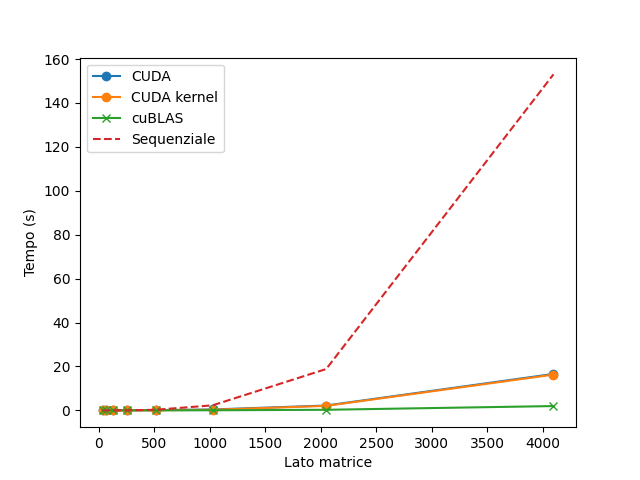
\includegraphics[width=0.6\textwidth]{./imgs/graphs/caso_0.png}
    \end{figure}
\end{frame}

\begin{frame}{Analisi}{Test - 1a}
    \begin{figure}[H]
        \centering
        \begin{minipage}{0.49\textwidth}
            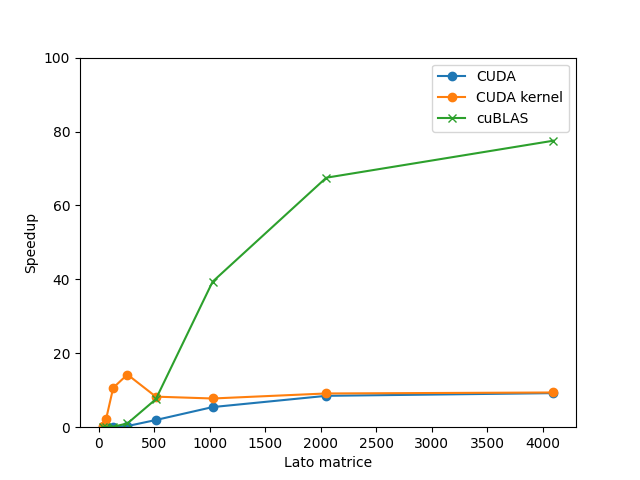
\includegraphics[width=\textwidth]{./imgs/graphs/caso_0_speedup.png}
        \end{minipage}
        \begin{minipage}{0.49\textwidth}
            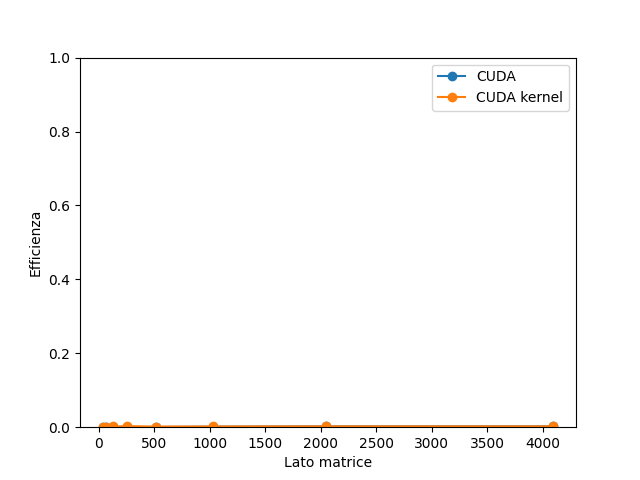
\includegraphics[width=\textwidth]{./imgs/graphs/caso_0_efficiency.png}
        \end{minipage}
    \end{figure}
\end{frame}

\begin{frame}{Analisi}{Test - 1b}
    \begin{enumerate}
        \item[1b] Aumentando i processi, a parità di thread (1024) e dimensioni della matrice ($2048 \times 2048$)
    \end{enumerate}

    \begin{figure}[H]
        \centering
        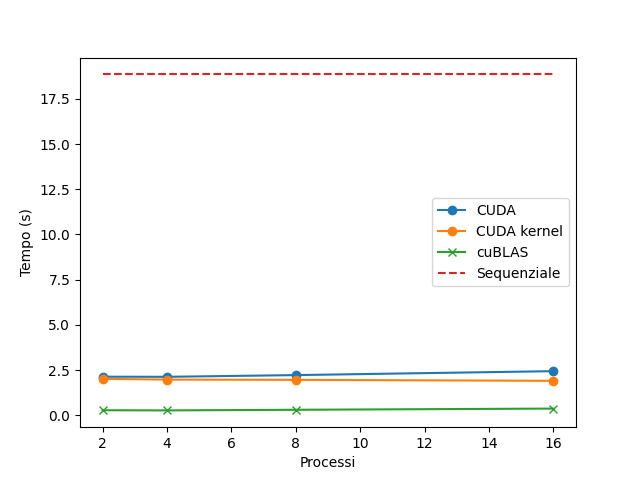
\includegraphics[width=0.6\textwidth]{./imgs/graphs/caso_a1.png}
    \end{figure}
\end{frame}

\begin{frame}{Analisi}{Test - 1b}
    \begin{figure}[H]
        \centering
        \begin{minipage}{0.49\textwidth}
            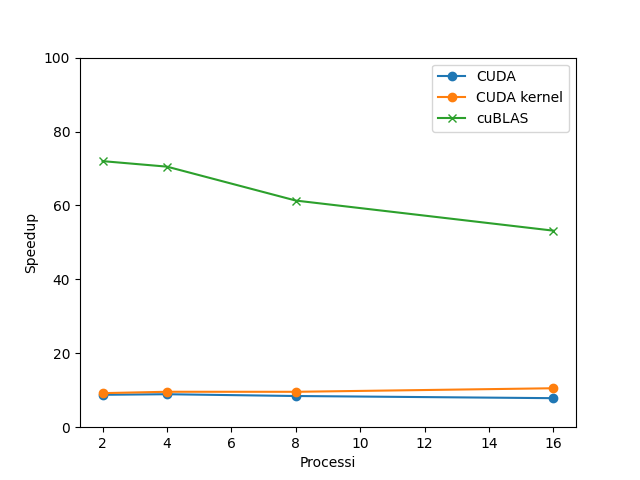
\includegraphics[width=\textwidth]{./imgs/graphs/caso_a1_speedup.png}
        \end{minipage}
        \begin{minipage}{0.49\textwidth}
            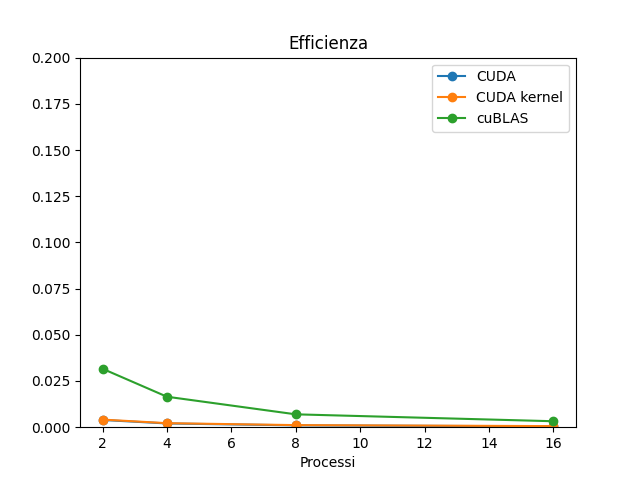
\includegraphics[width=\textwidth]{./imgs/graphs/caso_a1_efficiency.png}
        \end{minipage}
    \end{figure}
\end{frame}

\begin{frame}{Analisi}{Test - 1c}
    \begin{enumerate}
        \item[1c] Aumentando i thread, a parità di processi (4) e dimensioni della matrice ($2048 \times 2048$)
    \end{enumerate}

    \begin{figure}[H]
        \centering
        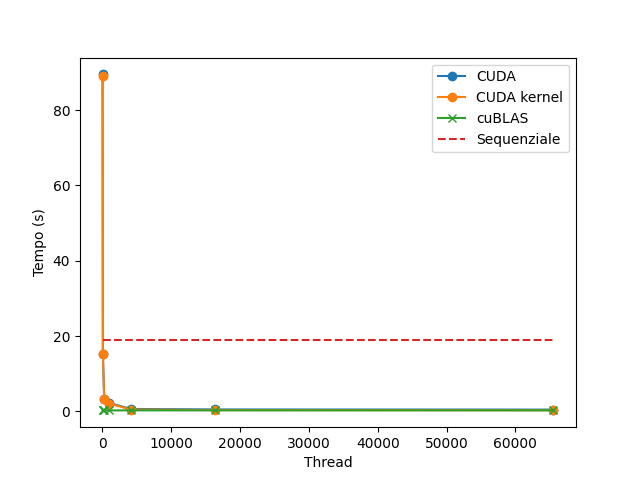
\includegraphics[width=0.6\textwidth]{./imgs/graphs/caso_a2.png}
    \end{figure}
\end{frame}

\begin{frame}{Analisi}{Test - 1c}
    \begin{figure}[H]
        \centering
        \begin{minipage}{0.49\textwidth}
            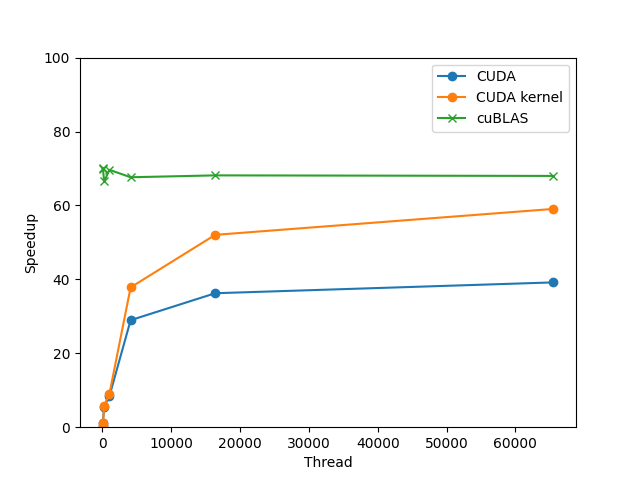
\includegraphics[width=\textwidth]{./imgs/graphs/caso_a2_speedup.png}
        \end{minipage}
        \begin{minipage}{0.49\textwidth}
            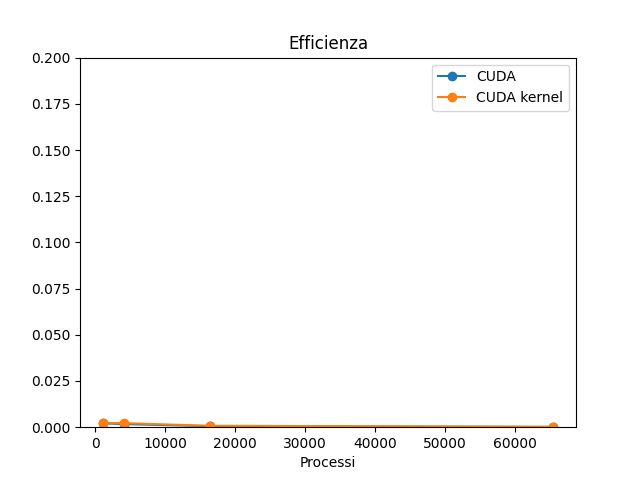
\includegraphics[width=\textwidth]{./imgs/graphs/caso_a2_efficiency.png}
        \end{minipage}
    \end{figure}
\end{frame}

\begin{frame}{Analisi}{Test - 2}
    \begin{enumerate}
        \item[2.] Aumentando i processi, a parità di thread ($1024 \times 1024$) e dimensione del problema \textbf{per processo} ($1024 \times 1024$)
    \end{enumerate}

    \begin{figure}[H]
        \centering
        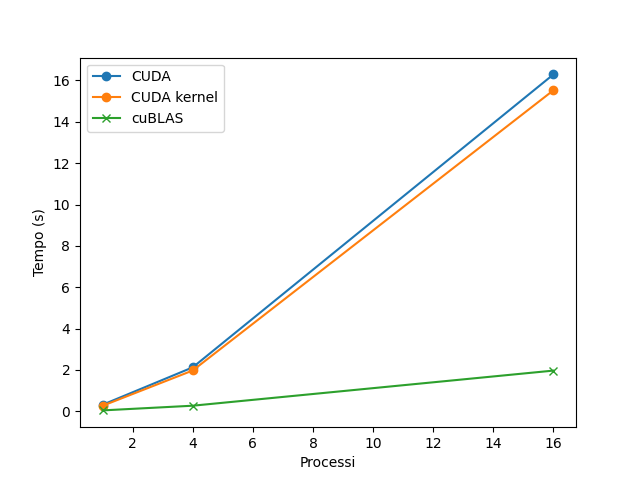
\includegraphics[width=0.6\textwidth]{./imgs/graphs/caso_b.png}
    \end{figure}
\end{frame}

\begin{frame}{Analisi}{Test - 2}
    \begin{figure}[H]
        \centering
        \begin{minipage}{0.49\textwidth}
            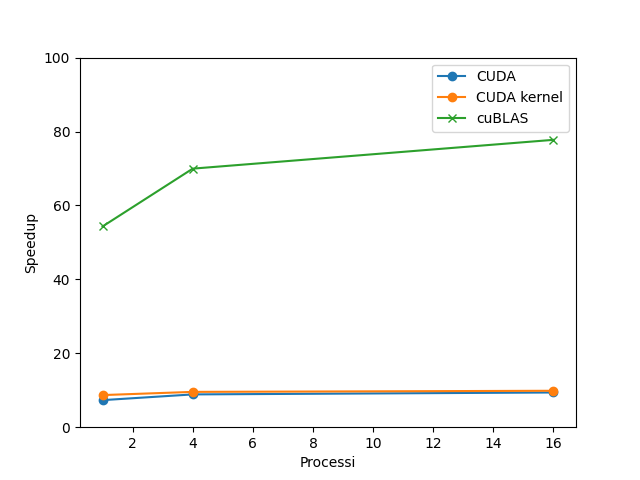
\includegraphics[width=\textwidth]{./imgs/graphs/caso_b_speedup.png}
        \end{minipage}
        \begin{minipage}{0.49\textwidth}
            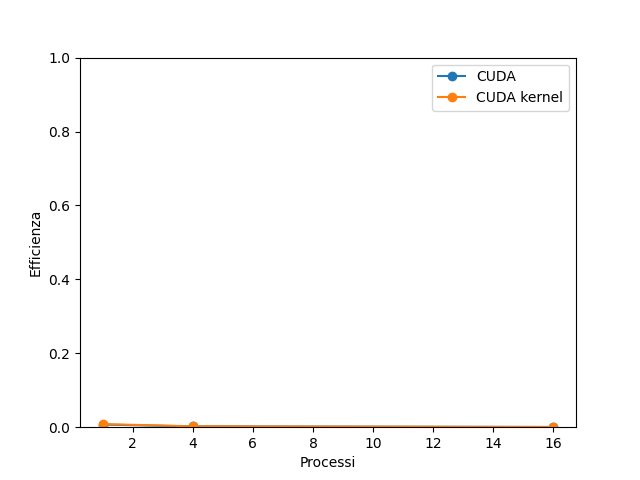
\includegraphics[width=\textwidth]{./imgs/graphs/caso_b_efficiency.png}
        \end{minipage}
    \end{figure}
\end{frame}

\begin{frame}{Analisi}{Test - 3}
    \begin{enumerate}
        \item[3.] Aumentando i thread, a parità di processi (4) e dimensione del problema \textbf{per thread}
    \end{enumerate}

    \begin{figure}[H]
        \centering
        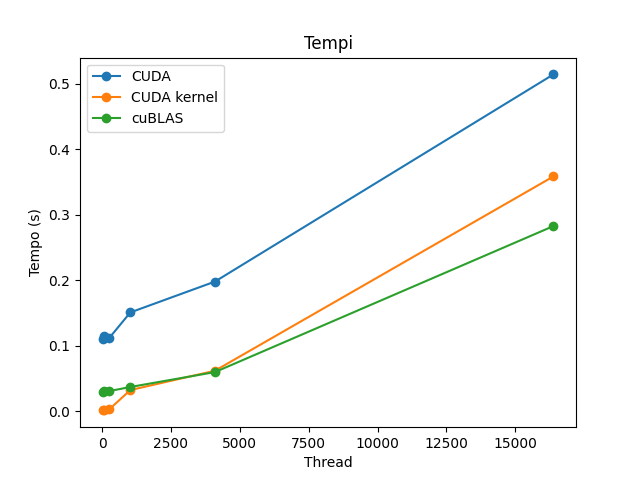
\includegraphics[width=0.6\textwidth]{./imgs/graphs/caso_c.png}
    \end{figure}
\end{frame}

\begin{frame}{Analisi}{Test - 3}
    \begin{figure}[H]
        \centering
        \begin{minipage}{0.49\textwidth}
            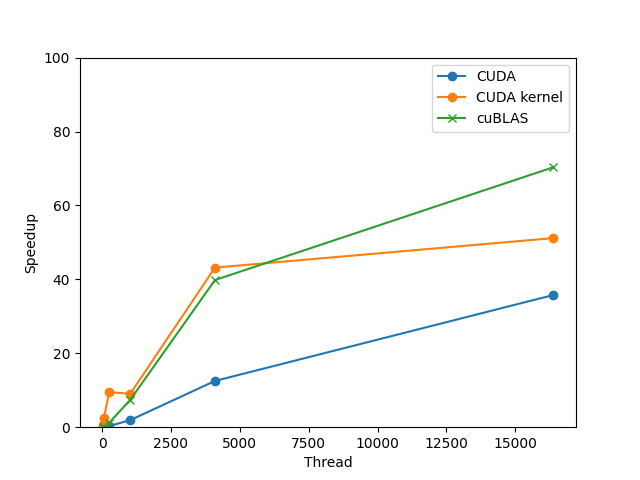
\includegraphics[width=\textwidth]{./imgs/graphs/caso_c_speedup.png}
        \end{minipage}
        \begin{minipage}{0.49\textwidth}
            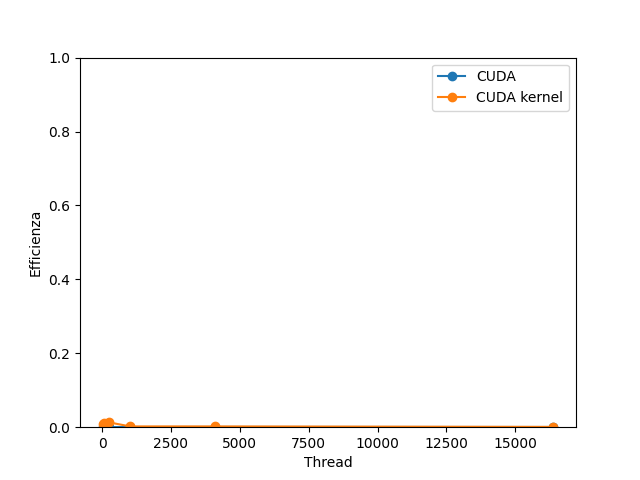
\includegraphics[width=\textwidth]{./imgs/graphs/caso_c_efficiency.png}
        \end{minipage}
    \end{figure}
\end{frame}

\begin{frame}{Analisi}{Test - 4}
    \begin{enumerate}
        \item[4.] Aumentando i processi, a parità di thread (1024) e dimensione del problema \textbf{per thread}
    \end{enumerate}

    \begin{figure}[H]
        \centering
        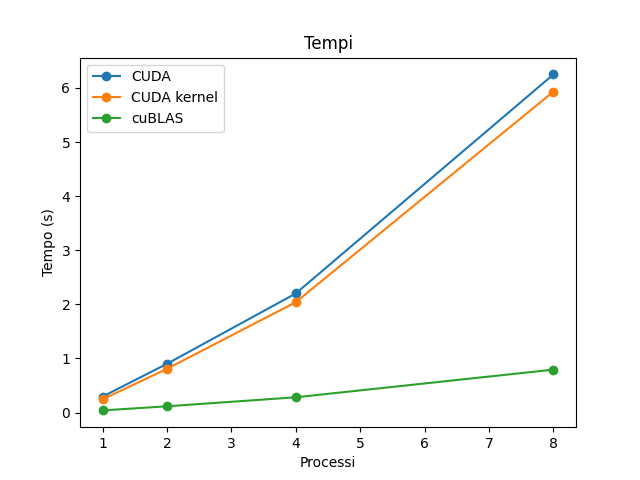
\includegraphics[width=0.6\textwidth]{./imgs/graphs/caso_d.png}
    \end{figure}
\end{frame}

\begin{frame}{Analisi}{Test - 4}
    \begin{figure}[H]
        \centering
        \begin{minipage}{0.48\textwidth}
            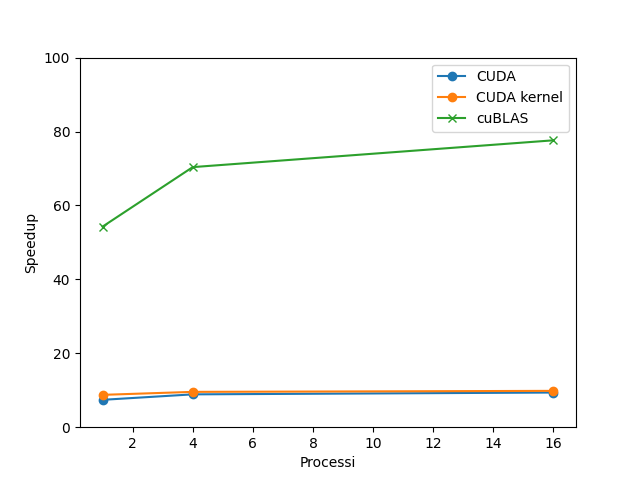
\includegraphics[width=\textwidth]{./imgs/graphs/caso_d_speedup.png}
        \end{minipage}
        \begin{minipage}{0.48\textwidth}
            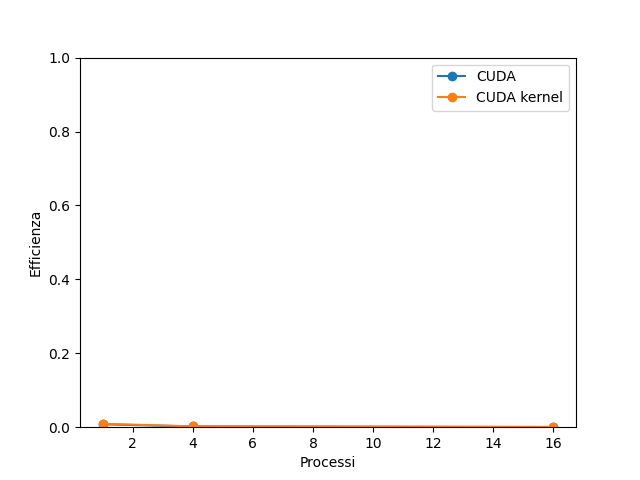
\includegraphics[width=\textwidth]{./imgs/graphs/caso_d_efficiency.png}
        \end{minipage}
    \end{figure}
\end{frame}

\begin{frame}{Analisi}{Conclusioni}
    \begin{itemize}
        \item Non vantaggioso per matrici piccole ($\approx 512 \times 512$)
        \item Aumentare thread più vantaggioso dell'aumentare i processi
        \item Overhead di comunicazione abbatte l'efficienza
    \end{itemize}
\end{frame}